\documentclass[11pt,a4paper]{article}
\usepackage[margin=1in]{geometry}
\usepackage[UTF8]{ctex}
\usepackage{amsmath,amssymb}
\usepackage{amsfonts}
\usepackage{graphicx}

\newtheorem{solution}{解答}
\renewcommand{\thesolution}{}

\title{分析力学第一次作业}
\author{张溢致\quad 致理数41\quad 2024011936}
\date{}

\begin{document}

\maketitle

\noindent \textbf{1.} 半径为 $R$ 的光滑半球形碗，固定在水平面上，一质量为 $m$ 的均质棒斜靠在碗缘，一端在碗内，一端在碗外，在碗内的长度为 $c$，如图1.4所示。试用虚功原理给出棒的全长。

\begin{solution}
以 $O$ 为原点，水平向左为 $x$ 轴、竖直向下为 $y$ 轴，棒与水平线的夹角为 $\theta$。圆心坐标为 $(R,0)$，故
根据集合关系自然有
\[
 c=2R\cos\theta.
\]
均质棒的质心 $G$ 距 $A$ 为 $L/2$，所以其向下坐标为
\[
 y_G=\left(c-\frac L2\right)\sin\theta
     =\left(2R\cos\theta-\frac L2\right)\sin\theta.
\]
只有重力作虚功。虚位移过程中 $L$ 固定，而 $c$ 随 $\theta$ 变化，因此平衡条件为
\[
 \delta W=mg\,\delta y_G
 =mg\left(2R\cos2\theta-\frac L2\cos\theta\right)\delta\theta=0.
\]
由 $\delta\theta$ 的任意性，得到
\[
 L=\frac{4R\cos2\theta}{\cos\theta}.
\]
代入 $\cos\theta=c/(2R)$，最终有
\[
 \mathord{L=4c-\frac{8R^2}{c}}.
\]


\end{solution}

\medskip
\noindent \textbf{3.} 在一半径为 $R$ 的竖直半圆硬钢丝上（两端点在水平线上），穿有质量分别为 $P$ 和 $Q$ 的两个小球，两球用长为 $2l$ 的不可伸长的轻绳相连，如图1.6所示。不计摩擦力，试用虚功原理求两球的平衡位置（即绳和水平线所成夹角 $\alpha$）。

\begin{center}
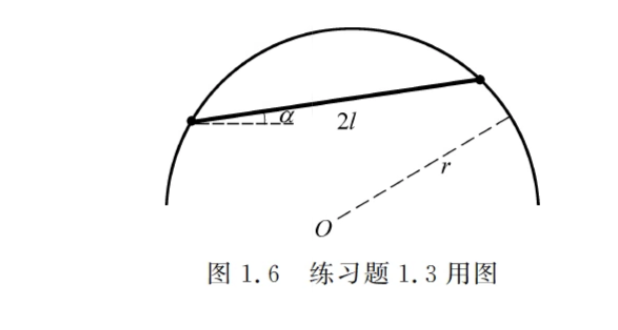
\includegraphics[width=6cm]{figures/fig1-6.png}
\end{center}

\begin{solution}
如图，两球位于上半圆，轻绳绷紧，设 $0<l<R$。取圆心 $O$ 为原点，竖直向上为 $y$ 轴。约定左球质量为 $P$，右球质量为 $Q$，绳从左向右上倾的有向角为 $\alpha$。

设绳的中点为 $C$，由圆心到弦中点的连线垂直于弦，得
\[
 OC=h=\sqrt{R^2-l^2}.
\]
$OC$ 与竖直向上的方向成 $\alpha$ 角，因此中点高度为 $y_C=h\cos\alpha$。两球的高度分别为
\[
 y_P=h\cos\alpha-l\sin\alpha,\qquad
 y_Q=h\cos\alpha+l\sin\alpha.
\]
钢丝光滑，支持力不作虚功；绳长不变，两端张力的总虚功为零。由虚功原理，平衡时有
\[
 -Pg\,\delta y_P-Qg\,\delta y_Q=0.
\]
取倾角的容许变化 $\delta\alpha$，则
\[
 \delta y_P=(-h\sin\alpha-l\cos\alpha)\delta\alpha,
\]
\[
 \delta y_Q=(-h\sin\alpha+l\cos\alpha)\delta\alpha.
\]
代入虚功方程，得到
\[
 g\bigl[(P+Q)h\sin\alpha+(P-Q)l\cos\alpha\bigr]\delta\alpha=0.
\]
由 $\delta\alpha$ 的任意性，
\[
 (P+Q)h\sin\alpha=(Q-P)l\cos\alpha.
\]
故在上述左右质量及有向角约定下，
\[
 \tan\alpha=\frac{(Q-P)l}{(P+Q)\sqrt{R^2-l^2}}.
\]
若将绳与水平线的夹角记为非负角 $\alpha_0$，则
\[
 \alpha_0=\arctan\!\left(\frac{|P-Q|\,l}{(P+Q)\sqrt{R^2-l^2}}\right).
\]
此上半圆内部平衡构型中，较重的小球位置较高；当 $P=Q$ 时，绳水平，两球关于竖直直径对称。
\end{solution}

\medskip
\noindent \textbf{5.} 质量为 $M$，倾角为 $\theta$ 的光滑斜面的底面放在光滑的水平面上，有一质量为 $m$ 的小块从顶端沿此斜面滑下，如图1.8所示。利用达朗贝尔原理，给出小块相对斜面的加速度。

\begin{center}
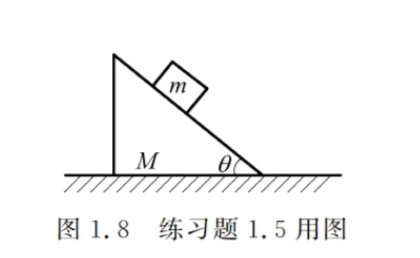
\includegraphics[width=4.8cm]{figures/fig1-8.png}
\end{center}

\begin{solution}
取水平向右为 $x$ 轴、竖直向上为 $y$ 轴。设斜面水平位移为 $X$，小块相对斜面沿斜面向下的位移为 $s$。于是小块的位置可写为
\[
 x_m=X+s\cos\theta,\qquad
 y_m=y_0-s\sin\theta,
\]
其中 $y_0$ 为常数。因斜面只作水平平移，所求相对加速度为 $\ddot s$，并有
\[
 \boldsymbol a_m=(\ddot X+\ddot s\cos\theta,-\ddot s\sin\theta),
 \qquad
 \boldsymbol a_M=(\ddot X,0).
\]
对应的容许虚位移为
\[
 \delta\boldsymbol r_m=(\delta X+\cos\theta\,\delta s,-\sin\theta\,\delta s),
 \qquad
 \delta\boldsymbol r_M=(\delta X,0).
\]
对“小块与斜面”整体应用达朗贝尔原理：
\[
 \sum_i(\boldsymbol F_i-m_i\boldsymbol a_i)\cdot\delta\boldsymbol r_i=0.
\]
地面支持力及斜面重力不作虚功；小块与斜面之间的法向作用力的总虚功为零。小块重力的虚功为 $mg\sin\theta\,\delta s$，因此
\[
 \begin{aligned}
 0={}&mg\sin\theta\,\delta s-M\ddot X\,\delta X\\
 &-m\Bigl[(\ddot X+\ddot s\cos\theta)
 (\delta X+\cos\theta\,\delta s)
 +\ddot s\sin^2\theta\,\delta s\Bigr].
 \end{aligned}
\]
按相互独立的 $\delta X$ 和 $\delta s$ 合并，得到
\[
 -\bigl[(M+m)\ddot X+m\ddot s\cos\theta\bigr]\delta X
 +m\bigl[g\sin\theta-\ddot X\cos\theta-\ddot s\bigr]\delta s=0.
\]
由虚位移的任意性，
\[
 \begin{cases}
 (M+m)\ddot X+m\ddot s\cos\theta=0,\\
 \ddot s+\ddot X\cos\theta=g\sin\theta.
 \end{cases}
\]
第一式给出 $\ddot X=-m\ddot s\cos\theta/(M+m)$。代入第二式可得
\[
 \ddot s\left(1-\frac{m\cos^2\theta}{M+m}\right)=g\sin\theta.
\]
故小块相对斜面的加速度为
\[
 \mathord{a_{\mathrm{rel}}=\ddot s
 =\frac{(M+m)g\sin\theta}{M+m\sin^2\theta}},
\]
方向沿斜面向下。
\end{solution}

\end{document}
